%!LW recipe=pdflatex

\documentclass[12pt,aspectratio=169]{beamer}
% \hypersetup{pdfpagemode=FullScreen}

\usepackage{upgreek}
\usefonttheme{professionalfonts}
\usepackage{mathtools}

\renewcommand*{\thefootnote}{\fnsymbol{footnote}}

\DeclareUnicodeCharacter{0301}{\'{e}}

\makeatletter
\def\onlyfootnote{\gdef\@thefnmark{}\@footnotetext}
\makeatother

\mode<presentation>
\useoutertheme[subsection=false]{miniframes}

\AtBeginSection[]{
    \begin{frame}
    \centering
    \begin{beamercolorbox}[sep=8pt,center,shadow=true,rounded=true]{title}
        \usebeamerfont{title}\insertsectionhead\par%
    \end{beamercolorbox}
    \end{frame}
}

\title{Apparate: Rethinking Early Exits to Tame Latency-Throughput Tensions in ML Serving}
\author{ \small
    Yinwei~Dai\inst{1,2}\and
    Rui~Pan\inst{1,2}\and
    Anand~Iyer\inst{2}\and
    Kai~Li\inst{1}\and
    Ravi~Netravali\inst{1}
}
\institute{
    \inst{1}Princeton University \\
    \inst{2}Georgia Institute of Technology
}
\date{Presenter: Shiwei Zhang}

\begin{document}
    \beamertemplatenavigationsymbolsempty

    \begin{frame}[plain]
        \titlepage
    \end{frame}



    \section*{Introduction}

    \begin{frame}
        \frametitle{Introduction}

        \begin{itemize}
            \setlength{\itemsep}{.8em}
            \item Machine Learning (ML) inference has become a staple for request handling in interactive applications
                  such as traffic analytics, chatbots, and web services
            \item Existing platforms impose harsh tradeoffs between \textbf{throughput} (cost) and \textbf{latency}.
            \item This paper explores \textbf{early exits (EE)} to resolve this tension.
        \end{itemize}
    \end{frame}



    \section{Background}

    \begin{frame}
        \frametitle{Throuphput-Latency Tradeoff}

        {
            \centering
            \includegraphics[page=2,trim=317.67bp 659.83bp 53.36bp 68.85bp,clip,scale=1.2]{apparate.pdf}
            \vskip .4em
        }

        Latency for an input is minimized by scheduling inference as soon as the request arrives with batch size of 1.
        \vskip .4em
        Throughput is maximized by creating large batches using a queuing system which directly inflates request
        latencies.
    \end{frame}

    \begin{frame}
        \frametitle{Early-Exit Models}

        EE inserts exit points (also called \textbf{ramps}) into the model to conditionally produce results without
        running some of the layers.

        {
            \vskip .8em
            \centering
            \includegraphics[page=2,trim=313.22bp 645.41bp 83.90bp 68.24bp,clip,scale=1]{eellm.pdf}
            \vskip .4em
        }

        For example, an object detection model do not need to run all layers to decide that there is nothing on an empty
        video frame.
        \vskip .4em
        Exiting decisions are made by comparing the entropy in the predicted result to a \textbf{threshold}.
    \end{frame}



    \section{Challenges}

    \begin{frame}
        \frametitle{C1: Latency and Resource Overheads}

        \begin{itemize}
            \setlength{\itemsep}{1em}
            \item The ramps take up GPU memory (6.56\% for BERT-Base).
            \item The additional exiting decisions increase latency of ``hard'' requests (up to 22\%).
        \end{itemize}
    \end{frame}

    \begin{frame}
        \frametitle{C2: Frequent and Costly Adaptation}

        \begin{columns}
            \begin{column}{0.5\textwidth}
                The optimal configurations (active ramps and their thresholds) changes frequently.

                \vskip 1.5em
                \includegraphics[page=4,trim=323.99bp 673.38bp 62.00bp 69.07bp,clip,scale=.85]{apparate.pdf}
            \end{column}
            \begin{column}{0.5\textwidth}
                \vskip -1.5em
                \centering
                \includegraphics[page=4,trim=55.90bp 553.68bp 318.45bp 71.97bp,clip,scale=.85]{apparate.pdf}
            \end{column}
        \end{columns}
    \end{frame}

    \begin{frame}
        \frametitle{C3: Lack of Accuracy Feedback}

        In production scenarios, serving optimizations that deliver accuracy reductions of more than 1-2\% are generally
        considered unacceptable. However, current EE proposals suffer from accuracy drops up to 23.9\%.

        \vskip 1em
        Once deployed, EE models do not provide indication of accuracy drops. When an exit is taken, the corresponding
        input does not pass throuput the remaining model layers, and the original model's prediction is never revealed.
    \end{frame}

    \begin{frame}
        \frametitle{C4: Incompatibility with batching}

        When inputs exit at ramps, the batch size for \textit{already scheduled tasks} shrinks, leading to resource
        underutilization for the rest of the execution.

        \vskip 1.5em
        \centering
        \includegraphics[page=3,trim=342.40bp 615.84bp 80.33bp 76.12bp,clip,scale=1.1]{apparate.pdf}
    \end{frame}



    \section{Design}

    \begin{frame}
        \frametitle{Key Design}

        Apparate focuses solely on latency savings by \textbf{allowing results to exit}, with \textbf{inputs still
        running to completion}.

        \vskip .5em
        \begin{itemize}
            \setlength{\itemsep}{.4em}
            \item Foregoing true exiting eliminates batch size changes during inference (C4).
            \item Running to completion grants Apparate with direct and continual feedback on accuracy (C3).
            \item This feedback provides the requisite information for continual adaptation of EE configurations (C1, C2).
        \end{itemize}
    \end{frame}

    \begin{frame}
        \frametitle{System Architecture}

        \centering
        \includegraphics[page=5,trim=54.22bp 570.53bp 320.28bp 69.24bp,clip,scale=1.1]{apparate.pdf}
    \end{frame}

    \begin{frame}
        \frametitle{Ramp Injection}

        Apparate considers layers that are \textit{cut vertices} as EE candidates.

        \vskip 1.5em
        \centering
        \includegraphics[page=5,trim=317.40bp 580.18bp 56.24bp 69.27bp,clip]{apparate.pdf}
    \end{frame}

    \begin{frame}
        \frametitle{Ramp Architectures}

        Apparate chooses many lightweight ramps instead of fewer expensive ramps.

        \vskip 1.5em
        \centering
        \includegraphics[page=6,trim=91.02bp 625.89bp 355.66bp 72.46bp,clip]{apparate.pdf}
    \end{frame}

    \begin{frame}
        \frametitle{Threshold Tuning}

        \textbf{Triggering:} Threshold tuning is triggered any time a window's accuracy falls below the user-specified
        accuracy constraint.

        \vskip 1em
        \textbf{Evaluation:} Apparate identifies the earliest ramp whose top prediction now has an error rate below its
        threshold and compare its result with the original model output.

        \vskip 1em
        \textbf{Greedy Search:} Based on the fact that \textit{higher thresholds result in monotonic decreases in
        accuracy and latency}, Apparate designs a hill climbing algorithm to decide the thresholds for active ramps.
    \end{frame}

    \begin{frame}
        \frametitle{Greedy Search}

        Starting with thresholds of 0 for all active ramps, Apparate choose a direction with largest \textbf{additional
        latency saving per unit of additional accuracy loss}. Apparate follows a \textbf{multiplicative increase,
        multiplicative decrease} policy on step size to balance search speed and granularity.


        \vskip .5em
        \centering
        \includegraphics[page=7,trim=60.00bp 576.10bp 325.36bp 70.56bp,clip,scale=.95]{apparate.pdf}
    \end{frame}

    \begin{frame}
        \frametitle{Ramp Adjustment}

        Apparate periodically adjusts the active ramps, which ultimately provides bounds on potential latency savings.

        \vskip 1em
        Unlike threshold tuning which runs reactively, ramp adjustment runs periodically. This is because threshold
        directly affects accuracy and must react promptly, while ramp adjustment only affects latency and is pure
        optimization. In addition, ramp adjustment requires deployments to evaluate the impact of new ramps.
    \end{frame}

    \begin{frame}
        \frametitle{Removing Active Ramps}

        Apparate defines the utility of ramp $\text{R} = \texttt{savings} - \texttt{overheads}$, where \texttt{savings}
        is the sum of raw latency that exiting inputs avoided by using R, and \texttt{overheads} is the sum of raw
        latency that R added to inputs that did not exit.

        \vskip 1em
        If any negative utility values exist, Apparate applies a fast threshold tuning round to see if ramp utilities
        become positive without harming overall latency savings. If not, Apparate deactivates all negative-utility
        ramps.
    \end{frame}

    \begin{frame}
        \frametitle{Adding New Ramps}

        \textbf{Intuition: } later ramps exhibit higher exit rates than earlier ones.

        \vskip 1em
        The upperbound exit rate is calculated as the sum of profiled exit rates for the following deactivated ramp and
        any earlier deactivations.

        {
        \vskip .5em
        \centering
        \includegraphics[page=8,trim=323.21bp 664.77bp 60.16bp 74.41bp,clip]{apparate.pdf}
        \vskip .5em
        }

        The ramp with the highest utility score is selected for trail.
    \end{frame}



    \section{Evaluation}

    \begin{frame}
        \frametitle{Setup}

        \begin{itemize}
            \setlength{\itemsep}{.8em}
            \item \textbf{Models}: 10 models across 4 families, covering CV and NLP.
            \item \textbf{Workloads}: CV workloads comprise real-time object classification on 8 one-hour videos. NLP
                                      workloads use Amazon product reviews and IMDB movie reviews.
            \item \textbf{Parameters}: SLO is 2x of each model's inference time with batch size 1. Accuracy constraint
                                       is 1\%. Ramp overhead budget is 2\% impact on worst-case latency.
            \item \textbf{Hardware}: Single machine with one NVIDIA A6000 and 32-core AMD CPU.
            \item \textbf{Platforms}: TensorFlow-Serving and Clockwork (using PyTorch).
        \end{itemize}
    \end{frame}

    \begin{frame}
        \frametitle{Comparison with Baselines}

        \centering
        \includegraphics[page=9,trim=317.75bp 641.14bp 54.69bp 72.62bp,clip]{apparate.pdf}
        \vskip 1em
        \includegraphics[page=10,trim=53.55bp 639.24bp 318.55bp 73.53bp,clip]{apparate.pdf}
    \end{frame}

    \begin{frame}
        \frametitle{Comparison with Existing EE Strategies}

        Existing EE approaches yield unacceptable accuracy drops while having longer tail latencies as compared to
        Apparate.

        \vskip 1em
        \centering
        \includegraphics[page=11,trim=317.01bp 509.80bp 54.01bp 189.35bp,clip]{apparate.pdf}
    \end{frame}

    \begin{frame}
        \frametitle{Microbenchmarks - Parameter Sensitivity}

        \centering
        \includegraphics[page=11,trim=319.82bp 364.52bp 57.17bp 331.39bp,clip,scale=.95]{apparate.pdf}
        \vskip 1.2em
        \includegraphics[page=12,trim=96.15bp 671.81bp 360.09bp 68.65bp,clip]{apparate.pdf}
    \end{frame}

    \begin{frame}
        \frametitle{Microbenchmarks - Ramp Architectures}

        When using DeeBERT's more expensive ramps, Apparate performs \textbf{4\% worse} since the costlier ramps
        constrain Apparate's runtime adaptation, i.e., \textbf{fewer active ramps} at a time.
    \end{frame}

    \begin{frame}
        \frametitle{Microbenchmarks - Impact of Serving Platform}

        The (median, p95) latency over vanilla models are similar on the two platforms.

        \vskip 1em
        \centering
        \includegraphics[page=12,trim=71.76bp 621.95bp 336.06bp 130.78bp,clip]{apparate.pdf}
    \end{frame}

    \begin{frame}
        \frametitle{Microbenchmarks - Profiling Apparate}

        Ramp adjustment rounds take 0.5ms. Additional CPU-GPU communication take 0.5ms, where 0.4ms comes from PCIe
        latencies.

        \vskip 1em
        \centering
        \includegraphics[page=7,trim=318.13bp 631.29bp 175.56bp 71.07bp,clip]{apparate.pdf}
    \end{frame}

    \begin{frame}
        \frametitle{Microbenchmarks - Ablation Study}

        Disabling ramp adjustment results in 20.8-33.4\% lower median latency wins.
    \end{frame}


    \section{Conclusion}

    \begin{frame}
        \frametitle{Conclusion}

        Strength:

        \begin{itemize}
            \setlength{\itemsep}{.4em}
            \item Coherent design around a novel idea (running EE models to completion).
            \item Automatic and non-intrusive system (no modification on model definition and serving platform).
        \end{itemize}

        \vskip 1em
        Limitation:

        \begin{itemize}
            \setlength{\itemsep}{.4em}
            \item The paper motivates with the throughput-latency tradeoff, but the proposed solution is
                  accuracy-latency tradeoff.
            \item Limited to time-related tasks.
            \item Early returning results for some samples may not always be meaningful. e.g., during LLM decoding.
        \end{itemize}
    \end{frame}

    \begin{frame}
        \frametitle{Takeaways}

        \begin{itemize}
            \setlength{\itemsep}{.4em}
            \item EE may be promising in cutting the cost of large models serving.
            \item Workload-specific optimization can be very powerful. e.g., vLLM's design for beam search.
            \item An idea: combine with pipeline parallelism?
        \end{itemize}
    \end{frame}

    \appendix

    \begin{frame}
        \vskip 1em

        \centering \huge
        Thank you!
    \end{frame}

    \begin{frame}
        \frametitle{Training and Deployment}

        Apparate prohibits early exits during initial training, ensuring that ramps are trained independently. This is
        because Apparate will adaptively change the active ramps at runtime.

        \vskip 1em
        For initial deployment, Apparate evently space the ramps based on the budget and GPU memory. To avoid accuracy
        dips, all ramps begin with thresholds of 0, i.e., no exiting.
    \end{frame}
\end{document}
